\documentclass{style}

%%%%%% acronyms %%%%%%
\usepackage[acronym,toc]{glossaries}
\newacronym{MIT}{MIT}{the Massachusetts Institute of Technology}
\newacronym{UW}{UW}{University of Wisconsin}
%\newacronym{<++>}{<++>}{<++>}
\makeglossaries

\usepackage[printwatermark]{xwatermark}
\usepackage{xcolor}
\newwatermark[allpages,color=black!5,angle=45,scale=6,xpos=-40,ypos=40]{DRAFT}

%%%%%%%% cover info %%%%%%%%%%%%%%%
\title{Facility and Time Step Discretization Effects in Fuel Cycle Simulation}
\author{Robert~W.~Carlsen, Paul~P.H.~Wilson}

\institute{University of Wisconsin - Madison, Department of Nuclear Engineering and Engineering Physics, Madison, WI 53706}
\submitter{Robert W. Carlsen}
\submitteraddress{229 N Midvale Blvd Apt 1, Madison, WI 53705}
\submitteremail{rwcarlsen@gmail.com}

% No more than three keywords, though each can be a phrase
\keywords{nuclear fuel cycle, simulation, TODO:third}

%%%%%%%%% includes and commands %%%%%%%%%%

\usepackage{graphicx}
\usepackage{placeins}
\usepackage{tabularx}
\usepackage{booktabs} % nice rules for tables
\usepackage{microtype} % if using PDF
\usepackage{xspace}
\usepackage{hyperref}
\usepackage{caption}
\usepackage{cite} % order citations correctly
\usepackage{float} % used to help position figures with the H modifier

\newcommand{\Cyclus}{\textsc{Cyclus}\xspace}%
\newcommand{\Cycamore}{\textsc{Cycamore}\xspace}%
\date{}

%%%%%%%%%%%%%%%%%%%%%%%%%%%%%%%%%%%
\begin{document}

\newpage
\begin{abstract}
TODO: Write this abstract.
\end{abstract}

\section{Introduction}

\subsection{Motivation and Background}

Due to the diversity of fuel cycle simulators' modeling assumptions direct
comparison and benchmarking can be difficult.  In 2012 the Organisation for
Economic Co-operation and Development (OECD) completed a benchmark study
\cite{oecd2012benchmark} that is perhaps one of the most complete published
comparisons performed.  Despite this, however, various results from the
different simulators were often significantly different due to different
modeling decisions such as reprocessing strategies, refueling behavior,
reactor end-of-life handling, etc.

Traditionally, many fuel cycle simulators have used a system dynamics approach
\cite{forrester_industrial_1961} to modeling. These simulators model several
"stocks" that have levels that change over time due to "flows" between them.
The flows are determined by an equation that is a function of the state of the
system (i.e. the system's stocks).  A constructed system is then solved
in discrete or continuous time depending on the limitations of the software
and constraints imposed by the model.  In system dynamics simulators, the
number of stocks and potential flows between them is generally a static
property of the modeled system, making it more difficult to swap different
reactor models in and out of the same scenario without wiring them into the
simulator manually.

System dynamics based fuel cycle simulators generally use a collection of
stocks to represent the state of groups of like facilities commonly referred
to as "fleets".  As the simulation steps through time, the levels of stocks
(e.g. reactor fresh fuel inventory, repository waste inventories, etc.) are
adjusted according to the calculated flow values.  Simulators that model
facility fleets built on a system dynamics foundation include VISION
\cite{jacobson_verifiable_2010}, DANESS \cite{van_den_durpel_daness_2009},
DYMOND (predecessor to DANESS), and ORION \cite{gregg_orion_2012} among
others.  In fleet-based modeling:

\begin{itemize}

    \item groups of facilities (usually all facilities of a given type) are
    treated as a single, aggregate entity.

    \item resource flows are often (approximately) continuous (limited by time
        step discretization)

\end{itemize}

This work investigates in detail differences between fleet vs. individual
reactor modeling.  The difference between these two modeling styles in terms
of their affects on output of fuel cycle simulators in general is currently
unknown. This analysis is designed to provide both quantitative and
qualitative insight about how fleet-based continuous flow models differ from
individual facility discrete flow models.

Many fuel cycle simulators step through time in discrete steps.  The duration
of a single time step can have significant impact on the dynamics of a
simulation.  The time step duration can affect the magnitude of individual
material transfers between facilities and correspondingly affects the noise
level in facility material inventories.  It can also act as a minimum bound
for outage durations. The effects of the time step duration will also be
investigated together with fleet vs facility modeling.

Questions of interest include:

\begin{itemize}

    \item How well do fleet-based models with continuous material flow capture
    optimal fuel cycle transitions compared to individual facility modeling?

    \item What effects are the primary drivers for differences in fleet-based
    and individual-based facility modeling?

    \item Does the impact of time step duration changes differ in fleet-based
    and individual-based facility modeling?

\end{itemize}

\subsection{CYCLUS}

One of the major motivations for the development of the Cyclus fuel cycle
simulator \cite{cyclus_2015} was creating a simulation environment that is
more expressive than more traditional fuel cycle simulators.  Cyclus was
designed with a plugin-style architecture that allows different models for
facility types to be swapped in and out trivially.  As a Cyclus simulation
walks through each time step, facilities engage in a market-like dynamic
resource exchange (DRE).  They broadcast requests for material and suppliers
respond with bids. The DRE then creates a network flow problem that it
optimizes to resolve which transactions actually occur.  The plugin
architecture combined with the DRE creates a powerful and flexible environment
for the natural comparison of different modeling paradigms.

Cyclus' agent-based architecture in concert with its dynamic resource exchange
has the ability to model fleet-based facilities.  However, Cyclus was designed
to enable modeling facilities individually with discrete flows enabling the
investigation of interesting real-world effects such as competition, reactor
cycle staggering, and individual reactor outages.  

\section{Methodology}

A single fuel cycle transition scenario is used with a few modeling variations
resulting in four different cases:

\begin{itemize}

    \item \emph{Case 1}: Monthly time steps with individual reactor modeling
    \item \emph{Case 2}: Monthly time steps with fleet reactor modeling
    \item \emph{Case 3}: Quarterly (3-month) time steps with individual reactor modeling
    \item \emph{Case 4}: Quarterly (3-month) time steps with fleet reactor modeling

\end{itemize}

Conducting this analysis involved developing some additional capability
in/around Cyclus.  Three primary pieces to the methodology are:

\begin{itemize}

    \item A fleet-based reactor model.

    \item A simulation scenario with both initial conditions and transition
        details.

    \item Theory and metrics for comparing differences between the four cases.

\end{itemize}

Because the standard package included with Cyclus does not include a
fleet-based reactor model, one was necessarily developed. A simulation
scenario was created that is roughly based on prior and ongoing work in the
Department of Energy (DOE).  A few Phenomena related to the different modeling
choices in each of the four cases are identified and used as a basis for
comparison.  Each of these three things is described in more detail in the
following sections.

\subsection{Fleet Reactor Implementation}

A fleet reactor facility was created for Cyclus.  The flexibility of Cyclus
makes it relatively straight forward to create plug-in models for Cyclus that
live anywhere along the spectrum from individual, discrete facilities to
continuous flow fleet facilities.  In order to contrast well with individual,
single-facility granularity modeling, the fleet model created here falls more
toward the aggregate, continuous flow side of the spectrum.  

The fleet reactor, although a single entity modeling many reactors, is
actually designed to look like many individual reactors to the cyclus
simulator kernel. This "trick" allows other plugins for managing facility
deployments to transparently work with the fleet reactor without having to
know anything about the fleet concept.  The fleet reactor has several
important characteristics described below:

\begin{itemize}

    \item Reactor capacity is deployed and retired in single reactor units
        (e.g. 1 GWe LWRs).

    \item Material is discharged from the fleet's reactor cores continuously
        (every time step) according to the following equation:

        \begin{equation}
            D =
            \frac{B}{L} \cdot N_{r} \cdot \frac{C_{inv}}{C_{cap}}
            \label{eqn:fleet-discharge}
        \end{equation}

        $D$ is the discharge rate (kg per time step), $B$ is the batch size
        (kg) for a single reactor's batch, $L$ is the cycle length (including
        refueling time) in time steps, $N_{r}$ is the number of
        reactors in the fleet, $C_{inv}$ is the total amount of fuel in all
        reactor cores (kg), and $C_{cap}$ is the total fuel capacity for all
        reactor cores (kg).  The last fraction term accounts for any amount of
        underfueling that may be occuring resulting in lower fuel burning
        rates due to unfueled reactors.

    \item Refueling occurs continuously with as much fresh fuel as is
        available up to the total amount to fill all reactor cores in the
        fleet.

    \item Generated power is computed similarly to core discharge rates by
        multiplying the total fleet power capacity by the same last term of
        Equation \ref{eqn:fleet-discharge} to account for unfueled capacity in
        the fleet.

    \item When a reactor in the fleet is retired, a full core of material is
        discharged - even if there is some fraction the fleet with unfueled
        cores.
        
\end{itemize}

These characteristics result in a fleet reactor having perfect fuel sharing
and perfect cycle staggering among the individual reactors it models.  First
discharge of spent fuel from fleets begins immediately rather than after a
complete refueling cycle. Fuel shortages also only cause proportional loss of
capacity rather than whole-reactor quantized shutdown.  The full
implementation of the fleet-based reactor is publicy available for download
\cite{Carlsen2015}.

\subsection{Scenario Description}

The scenario used is a transition from a the current once-through light water
reactor (LWR) fleet to a full sodium fast reactor (SFR) fuel cycle known as
EG-23 in the DOE's Advanced Nuclear Fuel Cycle Options report
\cite{wigeland_nuclear_2014}. Scenario and transition details were patterned
after ongoing work by the DOE in their Fuel Cycle Options campaign.

The scenario starts with 100 LWRs and follows an exponential curve with a 1\%
annual growth rate for 200 years.  The decommissioning of the initial 100
reactors is staggered over years 15 to 55.  Enrichment feeds LWRs with fresh
fuel with infinite capacity. In year 35, fast reactors become available for
deployment and no more thermal reactors are built.  LWR spent fuel separations
begins in year 15 with 2000 MTHM/yr capacity and increases to 3000 MTHM/yr in
year 25.  Fast reactor spent fuel separations and fuel fabrication have
infinite capacity.  All spent fuel is stored/cooled for 7 years before it is
available for separations. Figure \ref{fig:flow} shows the material flow
relationships between the facilities.  Compositions used for the simulations
were simple, containing primarily $^{238}U$, $^{235}U$, $^{239}Pu$,
$^{241}Am$, and small quantities of a few lanthanides.

\begin{figure}[!h]
    \centering
    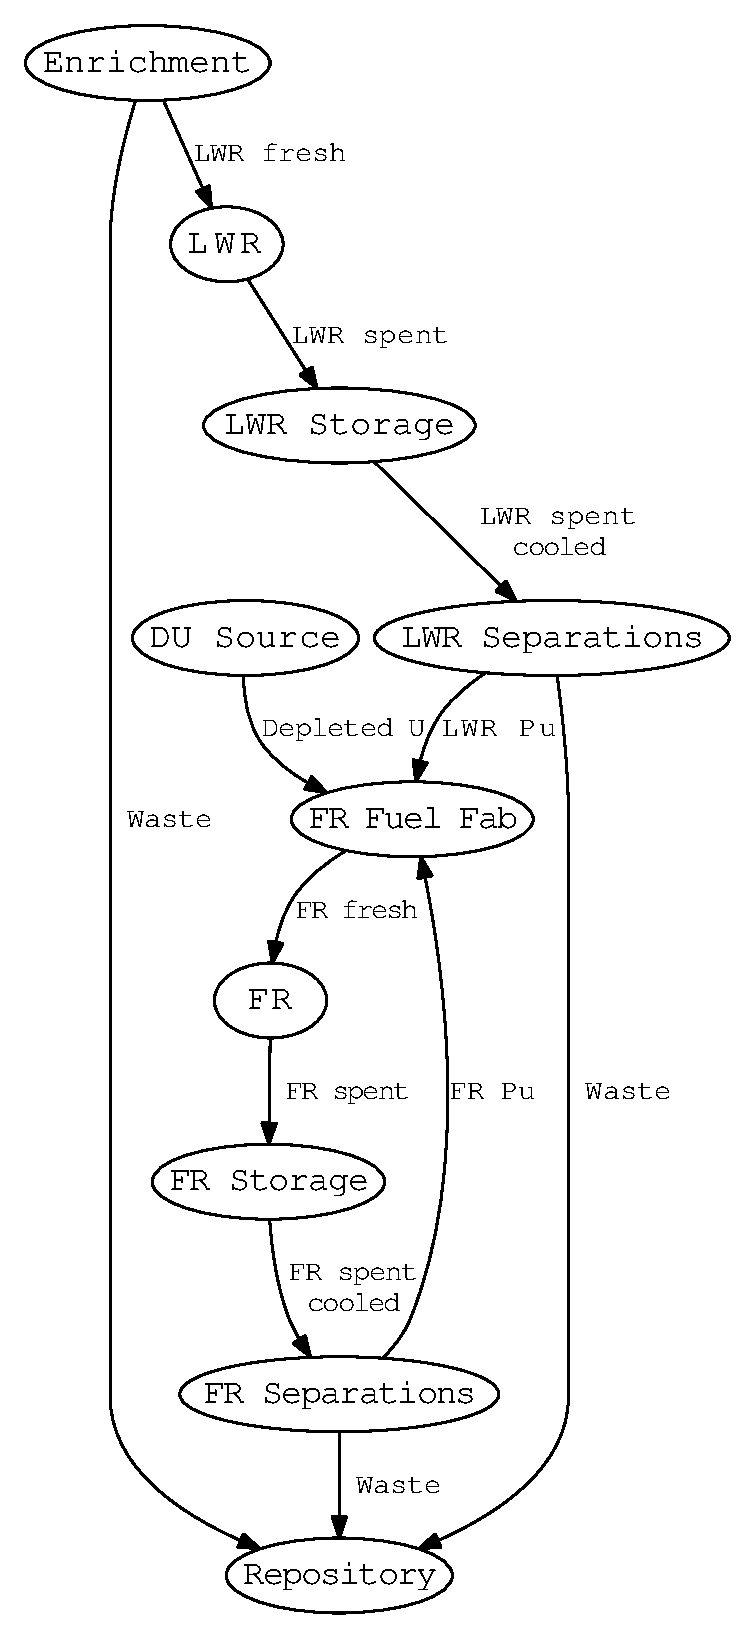
\includegraphics[width=0.47\textwidth]{exp2/flow.eps}
    \caption[Material flow paths]{Potential material flow paths between facility types.}
    \label{fig:flow}
\end{figure}

Cyclus version ?.? (TODO:~update~version) was used for this analysis.
Facility models used were the standard ones provided with Cyclus in the
Cycamore library (also version ?.?).  A custom storage facility was used
because Cycamore does not yet provide one.  The standard cycamore reactor was
used for both reactor types (LWR and SFR) in cases 1 and 3, and the custom
fleet-based reactor described earlier also used in cases 2 and 4.
Additional parameters for the reactor types are shown in Table
\ref{tab:reactors}.

\vspace{2mm}

\begin{table}[h]
    \centering
    \begin{tabular}{ |r | c c | }
        \hline                       
            & LWR & FR \\
        \hline                       
        Lifetime (yr)         & 80 & 80 \\
        Cycle length (months) & 18 & 14 \\
        Batch size (kg)       & 29565 & 7490 \\
        Batches per core      & 3 & 5 \\
        \hline                       
    \end{tabular}
    \captionsetup{justification=centering}
    \caption[Reactor facility parameters]{Reactor facility parameters. The cycle length includes the refueling outage.}
    \label{tab:reactors}
\end{table}

The described scenario is used as closely as possible in each of the four
cases.  However, a few other small case-dependent changes to the scenario
relating to reactor configuration are necessary.  For the cases using
quarterly time steps with individual reactors, cycle and outage times must be
adjusted to be a multiple of 3 months.  In order to make the comparison more
fair, the cases with monthly time steps are also adjusted to have identical
cycle and outage times.  The invariants preserved with respect to reactor
behavior are shown in Table \ref{tab:invar}.  Table \ref{tab:reactors} shows
the computed/selected configuration for both reactor types for all four cases.

\begin{table}
    \centering
    \begin{tabular}{ |r | c c | }
        \hline                       
                                                                             & LWR      & SFR      \\
        \hline                       
                                                                             &          &          \\
        Discharge Rate ($\frac{\text{kg} \cdot \text{HM}}{\text{month}}$)           & 1642.5   & 535      \\
                                                                             &          &          \\
        Burnup  ($\frac{\text{MWe} \cdot \text{month}}{\text{kg} \cdot \text{HM}}$) & 0.547945 & 0.672897 \\
                                                                             &          &          \\
        Effective Power  ($\text{MWe}$)                                      & 900      & 360      \\
                                                                             &          &          \\
        Core Size  ($\text{kg} \cdot \text{HM}$)                                    & 88695    & 40125    \\
                                                                             &          &          \\
        \hline                       
    \end{tabular}
    \captionsetup{justification=centering}
    \caption[Reactor parameter invariants]{
        Reactor configuration invariants maintained across all four
        simulation cases.
    }

    \label{tab:invar}
\end{table}

\begin{table*}
    \centering
    \begin{tabular}{ |r | c c | c c | }
        \hline                       
                                          & \multicolumn{2}{c |}{LWR}       & \multicolumn{2}{c |}{SFR} \\
                                          & Cases 1,3 & Cases 2,4 (fleet) & Cases 1,3 & Cases 2,4 (fleet)  \\
        \hline                       
        Cycle length (months)             & 15        & 18                & 12        & 15 \\
        Refueling outage (months)         & 3         & 0                 & 3         & 0 \\
        Batch size ($\text{kg} \cdot \text{HM}$) & 29,565    & 29,565            & 8,025     & 40,125 \\
        Power capacity (MWe)              & 1,080     & 900               & 450       & 360 \\
        \hline                       
    \end{tabular}
    \captionsetup{justification=centering}
    \caption[Reactor parameters by case]{
        Reactor configuration for each of the four simulation cases.
    }

    \label{tab:reactors}
\end{table*}

In each of the four cases, the initial 100 LWRs are modified to have a zero
length refueling outage with an explicit 900 MWe power capacity.  This was
done to avoid having all the initial LWRs in the individual reactor cases
refuel at the same time.  The parameters for each case were also selected to
keep capacity factors for individual reactors very roughly around 90\%.

A longer 21-month deployment period is used because it provides better natural
staggering for the reactor refueling cycles. The same deployment schedule is
used for all four cases; power capacity is built along a curve starting at
100GWe in year zero following the 1\% exponential growth curve.  This
particular deployment schedule causes significant fuel shortages providing
interesting features to investigate and compare.

The input files and other assets used in the analysis for each of the four
cases are publicly available for download \cite{Carlsen2015}.

\subsection{Modeling Effects}

There are various low level phenomena that have potential to affect the larger
outcome of simulations with respect to facility modeling decisions. Several
effects are described below that result from fundamental differences between
these two modeling paradigms.

One difference between the fleet and individual facility modeling is the
\emph{quantized shutdown effect}.  If a fleet-based reactor modeling 3-batch
cores is short a half batch of fuel it will produce $\frac{5}{6}\cdot C$ of
power for that time step where $C$ is the power capacity of a single reactor
of the fleet (e.g. 1000 MWe).  If an individually modeled reactor is short a
half batch of fuel, then it will produce no power that time step.  Time step
duration can also have this effect.  For both fleet and individual reactor
modeling, power goes offline in full time step increments.  For example, if a
3-batch fleet based reactor is short $\frac{1}{2}$ batch of fuel with a 3
month time step, then it will produce $\frac{5}{6} \cdot 3 \text{mo} \cdot C $
of energy.  In contrast, a monthly time step might allow the same reactor to
produce $[\frac{5}{6} \cdot 1 \text{mo} + 2 \text{mo}] \cdot C $ of energy if
the fuel shortage actually ended after only 1 month.

Individually modeled reactors each have their own refueling cycles.  Depending
on how the refueling cycles and outages are staggered, power production can
vary significantly.  For example, if all reactors refuel at the same time,
then all reactors would be offline at the same time.  This is referred to as
the \emph{cycle staggering effect} and does not occur in fleet-based reactor
models.  An example of poor cycle staggering is shown in Figure
\ref{fig:sync-cycle}.  Poor staggering causes spikes of material supply and
demand that can lead to suboptimal resource utilization.  A fuel fabrication
facility might receive requests for new batches for every reactor all at once.
The reactors draw out inventory from the fuel fabrication facility together in
a large quantity of orders.  If the fabrication facility does not have enough
on hand, some number of reactors will need to wait until enough fuel can be
pumped through fabrication.  Avoiding such constraints would require the
fabrication facility to maintain suboptimally large on-hand inventories as a
contingency.

\begin{figure}[h]
    \centering
    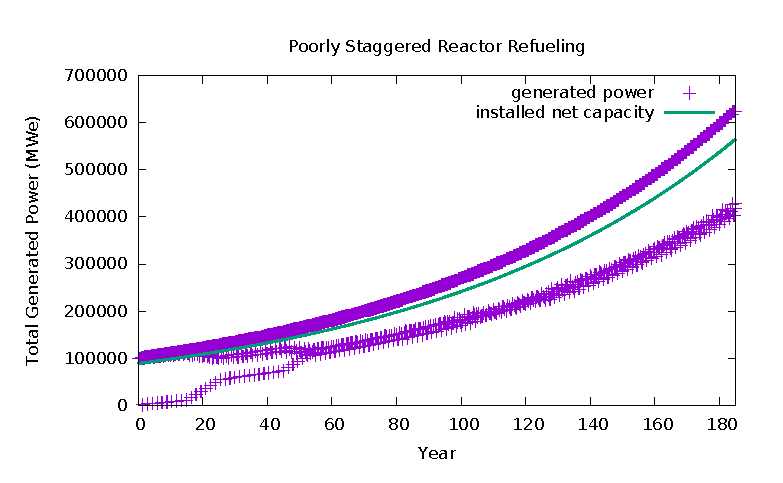
\includegraphics[width=1.0\columnwidth]{exp2/sync-cycle.eps}
    \caption[The cycle staggering effect]{
        In this scenario, reactors are deployed annualy with a refueling cycle
        length (including outage) of 18 months.  So all reactors deployed
        every 3rd year refuel together.  All initial 100 LWRs start out with
        their cycles synced as well.  While it may look like separate curves,
        this plot shows only a single time series.
    }
    \label{fig:sync-cycle}
\end{figure}

Another difference between fleet-based and individual facility modeling
involves fuel sharing.  Power production by a group of individual reactors for
a fixed amount of fuel shortage may vary depending on how the existing fuel is
distributed.  This is illustrated in Figure \ref{fig:fuel-sharing}.  A system
being short 3 batches might mean that one reactor has no batches and isn't
operating or that 3 reactors are each missing a single batch.  This is
referred to as the \emph{fuel sharing effect}.

\begin{figure}[h]
    \centering
    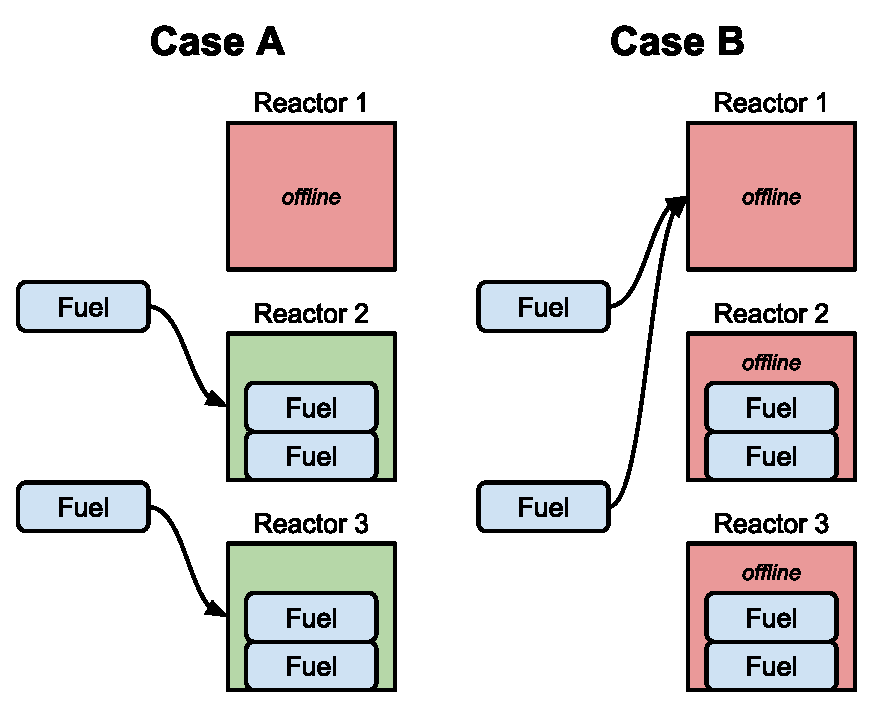
\includegraphics[width=0.8\columnwidth]{exp2/fuel-sharing.pdf}
    \caption[The fuel sharing effect]{
        A simple diagram showing effects of constrained fuel supply
        distribution choices. In both cases A and B, reactor 1 needs 3 new
        fuel batches to operate and reactors 2 and 3 each need 1 fresh batch.
        In case A, the two batches are given to reactors 2 and 3, resulting in
        reactor 1 remaining offline. In case B, the available fuel batches are
        given to reactor 1 resulting in all three reactors being offline.
    }
    \label{fig:fuel-sharing}
\end{figure}

One important phenomenon related to time step duration is the \emph{inventory
drawdown effect}.  Increasing time step duration reduces the frequency over
which refueling can occur, resulting in larger impulse drawdown on
inventories. This by itself is not problematic because this is balanced by
correspondingly larger inventory top-up quantities.  The other component of
this effect is the simultaneity of incoming and outgoing material flows on a
given time step.  Within a particular time step facilities do not know about
incoming material when they make commitments for outgoing material.  For
longer time steps, larger incoming quanta of material are not available for
making offers. In general longer time steps and individual reactor modeling
create a need for larger floating inventory buffers in order to avoid
material shortages.

There are also performance differences between the two modeling paradigms.  A
single 200 year simulation with several hundred fleet-based reactors takes
about 2 seconds to run on a typical desktop machine where the same simulation
using individual reactor facilities takes about 20 seconds.  This order of
magnitude difference is an important tradeoff to keep in mind when doing fuel
cycle analysis in general, particularly when considering optimization or
sensitivity studies where running hundreds of thousands of simulations may be
desirable.

\section{Results}

All results data, analysis tools and instructions are publicly available for
download at \url{http://dx.doi.org/10.6084/m9.figshare.1546775}
\cite{Carlsen2015}.

\subsection{Power Production}

Figure \ref{fig:power} shows an overall view of the generated
power over time for each of the four cases.  Figure
\ref{fig:power-rel} normalizes the Figure
\ref{fig:power} curves to the expected exponential power curve
magnifying some interesting differences between the four cases.  For the first
100 years, the four cases behave somewhat similarly, although the individually
modeled reactors in cases 1 and 3 actually go online and offline for refueling
causing more variance.  Around year 100, a fuel shortage begins and more
significant differences between the four cases become apparent. This fuel
shortage lasts until about year 140. The power generated in Case 4 is lower
than in case 2 during the fuel shortage years. This is primarily due to the
\emph{quantized shutdown effect}.  The longer 3-month time step in case 4
results in reactor capacity going offline longer than necessary.

During the initial 100 years, cases 1 and 3 have larger variance in power
output than cases 2 and 4.  This is caused by minor refueling cycle
synchronization.  The \emph{cycle staggering effect} becomes much more visible
during and after the fuel shortage as evidenced by the larger swings in power
generation from time step to time step.  Initially, the reactor cycles are
staggered well.  During the shortage, several reactors that previously had
staggered cycles are all offline together waiting for fuel.  On time steps
where reactors retire (not just during the shortage), new deployments are made
to replace them in addition to new deployments made to address power demand
growth.  Because the initial reactors retire in waves somewhat close together,
there are corresponding waves of deployment, and these waves are echoed every
80 years (the reactor lifetime).  These waves of deployment cause waves in
recycled fuel availability that cause many of the reactors offline during the
shortage to receive fuel and come online together.  The net effect is that the
fuel shortage degrades reactor cycle stagering overall.  As the simulation
continues, however, new reactors continue to be deployed and reactors with
synchornized cycles retire resulting in a gradual return to decent better
staggering visible by the end of the 200 years.

\begin{figure*}[!h]
    \centering
    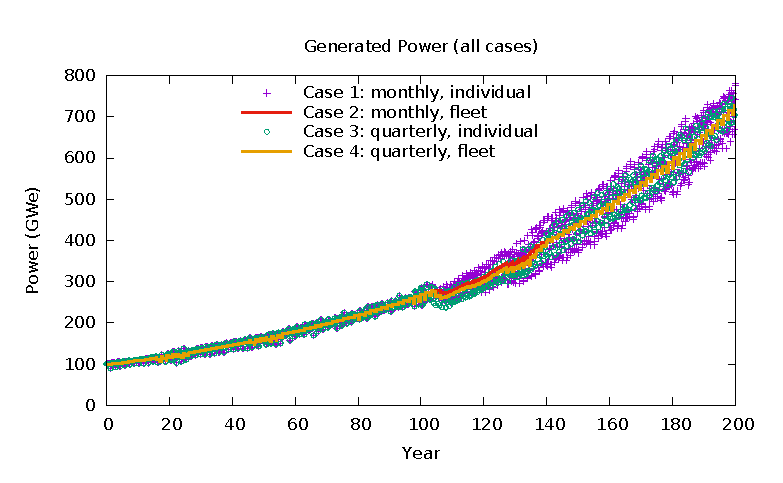
\includegraphics[width=0.8\textwidth]{exp2/power.eps}
    \caption[Generated power]{
        Generated power for all four cases.  A fuel shortage occurs from about
        year 100 to about year 140.  In cases 1 and 3 with individual reactor
        modeling, refueling cycles become much more synchronized during and
        after the fuel shortage resuting in large power fluctuations (the
        \emph{cycle staggering effect}).
    }
    \label{fig:power}
\end{figure*}

\begin{figure*}[!h]
    \centering
    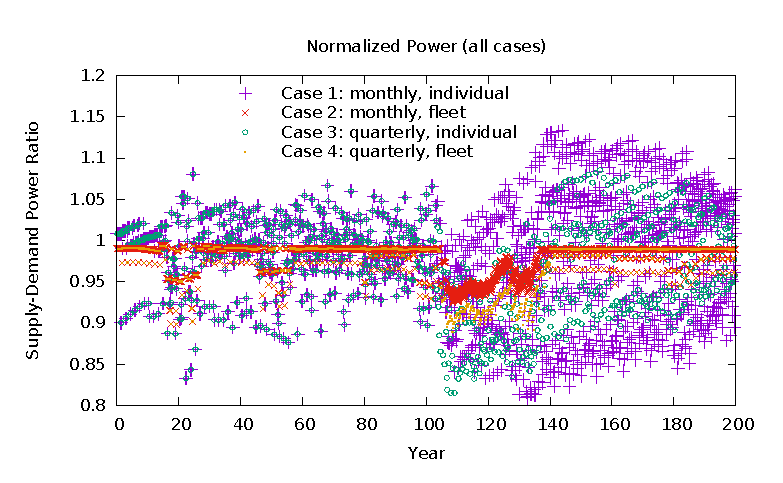
\includegraphics[width=0.8\textwidth]{exp2/power-rel.eps}
    \caption[Normalized power]{
        Generated power is normalized to the expected 1\% exponential growth
        curve for all four cases.  A fuel shortage occurs from about year 100
        to about year 140.  The \emph{cycle staggering effect} can be seen as
        divergence from 1.0 and is especially visible in cases 1 and 3 where
        the shortage increases cycle synchronization significantly. The
        \emph{quantized shutdown effect} can also be seen in the discrepency
        between quarterly and monthly time steps for fleet reactor modeling
        (cases 2 and 4) during the shortage; a longer time step causes more
        reactor outage than necessary. The consistent jumping up and down for
        the fleet reactor cases is due to the mis-alignment of reactors going
        offline (multiples of 12 months) and the build period (21 months).
    }
    \label{fig:power-rel}
\end{figure*}

\subsection{Fuel Shortage}

Figure \ref{fig:unfueled} shows the fuel shortage more explicitly
for each of the four cases. The individual reactor modeling cases result in
more cumulative outage than corresponding fleet-based cases. The quarterly
time step of cases 3 and 4 make the outage significantly more severe. Cases 1
and 3 exhibit approximately twice as much offline power as their corresponding
fleet based simulations in cases 2 and 4.  The monthly time step simulations
also have roughly twice as much offline power as their corresponding quarterly
cases.

\begin{figure}[!h]
    \centering
    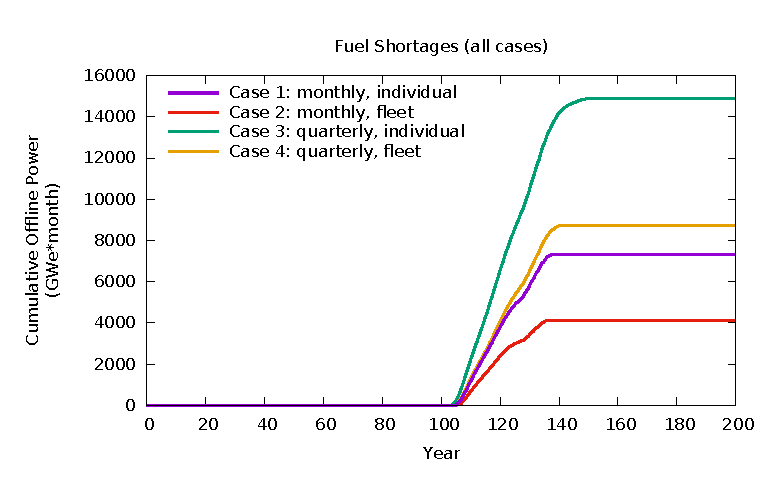
\includegraphics[width=1.0\columnwidth]{exp2/unfueled.eps}
    \caption[Cumulative offline power due to fuel shortage]{
        Cumulative offline power for reactors that had delayed cycle start due
        to fuel shortage. The difference between individual and fleet based
        modeling is primarily a result of the \emph{fuel sharing effect}. The
        difference between monthly and quarterly time steps is primarily
        caused by the \emph{inventory drawdown effect}.
    }
    \label{fig:unfueled}
\end{figure}

Quantifying imperfect fuel sharing is a bit difficult, but Figure
\ref{fig:badshare} gives one way to approximate the \emph{fuel
sharing effect}.  Fleet reactor modeling by design exhibits perfect fuel
sharing by design (zero inefficiency) and so is not included in this figure.
Every batch that is given to a reactor that ends up not being able to start it
cycle at the scheduled time (due to fuel shortage) adds one to this cumulative
for each time step the cycle start is delayed.

One useful over-estimate of the fuel sharing inefficiency is to assume every
one of these batches could have been given to a reactor enabling it to
operate.  Multiplying each of these cumulative batches by reactor capacity
(i.e. 450 MWe) provides a way to compare fuel sharing inefficiency with the
overall fuel outage.  Correcting for capacity factor in is appropriate these
cases because the outage is many reactor cycle lengths in duration. This
results in a cumulative offline power caused by poor fuel sharing of roughly
1,600 $\text{GWe} \cdot \text{months}$ and 5,400 $\text{GWe} \cdot
\text{months}$ for cases 1 and 3 respectively.  These approximations are a
significant portion of the difference between individual and fleet cases in
Figure \ref{fig:unfueled} suggesting that most of the discrepency
in cumulative outage between fleet and individual modeling is caused by
inefficient fuel sharing in the individual reactor cases.

The poor fuel sharing exhibited in the individual reactor cases would not
occur if there were no new reactors being built during the shortage.
Previously operating reactors only ever need one batch - receiving only a
single batch allows them to operate.  Newly constructed reactors need multiple
batches in order to begin operation, and if they receive less than a full core
they cannot operate.  The real world doesn't necessarily optimize for fuel
sharing efficiency very cleanly. There are other factors that can affect fuel
sharing outcomes.  A few include:

\begin{enumerate}

    \item Multiple fuel quanta comprise a single batch (i.e. multiple
        assemblies per batch). This functionality is natively supported in the
        individual reactor model.

    \item On-hand fresh fuel inventory maintained at reactors. This
        functionality is natively supported in the individual reactor model.

    \item Long-term fuel contracts between reactors operators and fuel
        suppliers.

\end{enumerate}

Having multiple assemblies per batch (item 1 above) will further degrade fuel
sharing efficiency.  Even reactors that are short only one batch could
potentially receive some fuel and still be unable to operate.  In order to
maintain optimal sharing, fresh fuel now needs to be sent in all-or-nothing
multi-assembly quanta with preference for reactors that need fewer assemblies.
Spare fresh fuel inventory (item 2 above) will have the global effect
increasing total outage severity; on average more batches of fresh fuel will
be sitting unused.  However, it can potentially reduce the frequency of
outages for individual reactors in some cases.

If they were to ever occur, real world fuel shortages would likely not result
in optimal fuel sharing. However, modeling these the causes of suboptimal fuel
sharing is probably best accomplished with a more direct, intentional approach
rather than as a modeling artifact as seen here in cases 1 and 3.  One way to
alleviate the poor fuel sharing is to modify the individual reactor model to
lower the preference value for requests for fresh fuel depending on how many
assemblies it needs to have a full core.  The more assemblies it needs, the
lower it will set its request preference.  This will have the effect of
allowing the resource exchange resolution in Cyclus to globally prefer sending
fuel to reactors that need less to operate.

\begin{figure}[!h]
    \centering
    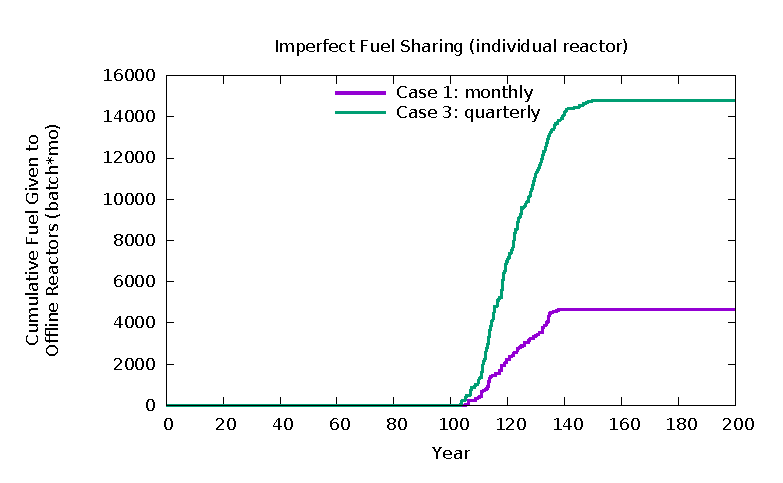
\includegraphics[width=1.0\columnwidth]{exp2/badshare.eps}
    \caption[Cumulative unnecessary idling fuel]{
        Fuel sharing inefficiency approximated by the cumulative number of
        fuel batches given to each reactor on each refueling period multiplied
        by the number of time steps that reactor had to delay the start of its
        next cycle (due to fuel shortage).  Fleet reactors have perfect fuel
        sharing by design and so are not included here. The large difference
        between cases 1 and 3 is mostly due to the \emph{inventory drawdown
        effect}. 
    }
    \label{fig:badshare}
\end{figure}

\subsection{Inventory Drawdown}

The large differences seen between monthly and quarterly time step cases in
Figures \ref{fig:unfueled} and \ref{fig:badshare} are
primarily caused by the \emph{inventory drawdown effect}.  Figure
\ref{fig:puinv} helps to visualize this effect.  The black dots in
the figure represent impulse flows of available Pu out of the fuel fab and
into fast reactors.  Blue lines represent the flows into Pu inventory
available for making fuel. The in flows are not shown for the individual
reactor cases because they are somewhat messy and obscure otherinformation in
the plots. The colored curves show Pu inventory available for making fast
reactor fuel.  When the inventory curves meet and force down the flows, fuel
shortages occur. 

Quarterly time steps have less frequent but larger impulse material flows.
These larger flows, however, do not compensate for the larger withdrawals
because facilities do not know about incoming inventory when they resolve
their outflow for a particular time step.  This information lag effectively
requires the floating Pu inventory to be maintained at a higher level.  This
can be clearly seen in the case 4 plot which has a higher standing inventory
than case 2 during the fuel shortage years.  The case 4 Pu inventory is unable
to drop below approximately 100 tonnes, which indicates out-flows to be
roughly equal to the Pu flow into inventory each time step during those years.
This can be confirmed by the in-flow and inventory curves touching at those
points.  Case 2 Pu inventory is similarly limited at about the 30 tonne level.
As expected, the case 4 withdrawals are also three times higher case 2
withdrawals.

\begin{figure*}[!h]
    \centering
    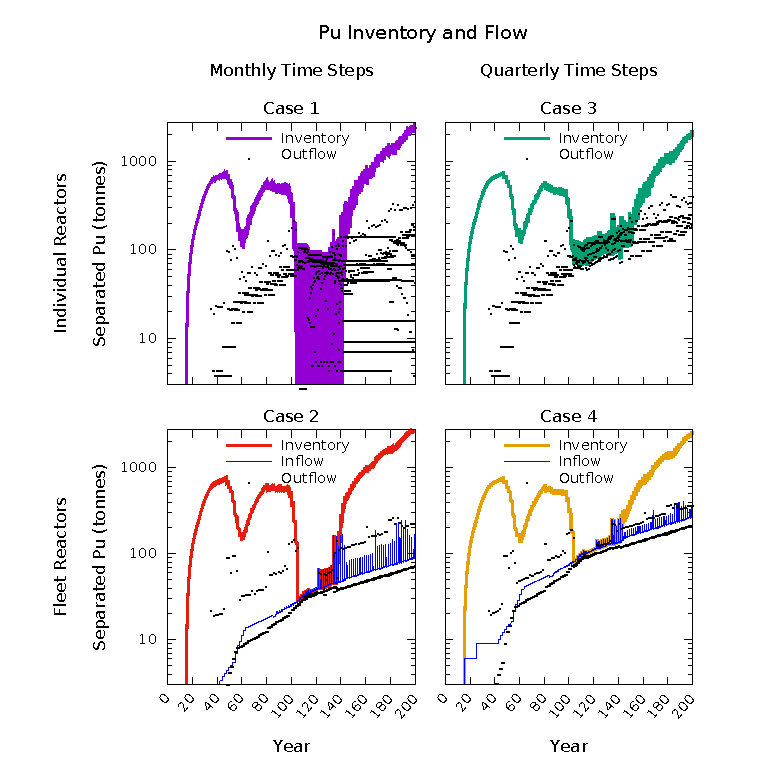
\includegraphics[width=1.0\textwidth]{exp2/puinv.eps}
    \caption[Pu inventory and flow]{
        Pu inventory and flows for all four cases.  In-flows for cases 1 and 3
        are omitted because they are very noisy and obscure useful other
        information.  Larger time steps results in larger per time step
        material flows. These larger flows mean more material is not available
        for supplying to requesters.  This information lag causes more supply
        constraints than occur with smaller time steps - illustrating the
        \emph{inventory drawdown effect}.
    }
    \label{fig:puinv}
\end{figure*}

Figure \ref{fig:puinv-compare} shows the same inventory curves from Figure
\ref{fig:puinv} superimposed. Counter-intuitively, lower separated plutonium
inventory during the shortage generally indicates fewer unfueled reactors.
Lower inventory levels mean available Pu is being utilized more efficiently
rather than sitting idle.  Cases 3 and 4 with their longer time steps show
higher inventories indicating a more severe shortage.  Post shortage, they
also fall a bit behind on building up Pu stocks due to the delayed
contributions of more unfueled reactors to the separated Pu pool.

\begin{figure*}[!h]
    \centering
    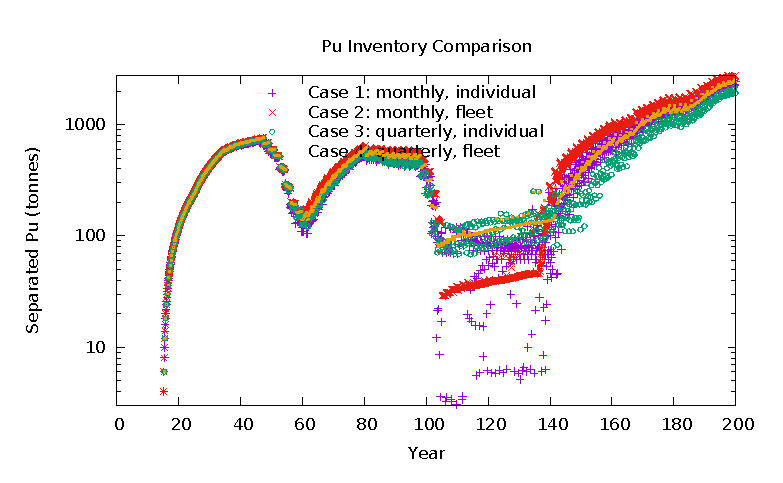
\includegraphics[width=0.8\textwidth]{exp2/puinv-compare.eps}
    \caption[TODO]{
        TODO
    }
    \label{fig:puinv-compare}
\end{figure*}

Also notable is that different modeling choices (e.g. time step duration,
facility discretization, etc.) may have varying levels of significance
depending on the scenario/context they are operating in.  As shown in Figure
\ref{fig:puinv-compare} Before the fuel shortage begins, differences between
each of the four cases are relatively minor.  However, after the shortage
begins around year 100, separated Pu inventories vary much more significantly
between the different cases.

\section{Conclusion}

Different modeling choices can have a significant impact on the outcome of a
simulation.  With discrete reactor modeling many factors must be considered in
order to ensure the integrity of conclusions.  Individual reactor outage
modeling can be very useful for certain analyses, but it can reduce result
quality if things such as cycle staggering are handled appropriately.  The
fleet and discreet modeling done here is itself multi-dimensional.  If
individual outages are not of interest, reactor power could be lowered and the
outage reduced to zero duration making the capacity factor part of the
reactor's power capacity.  The cycle staggering effects present when modeling
reactors individually can provide valuable insight not possible with the
fleet-based reactor modeling.  Starting reactors following shortage induced
outages should not follow the natural pacing of fuel availability, otherwise
refueling cycles become unsatisfactorily synchronized.

Increasing the time steps increases facilities' standing inventory requirement
for avoiding supply constraints.  Facilities that have unconstrained supply
and very large inventory buffers, are not affected by the time step in this
way.  Facilities can provide no more inventory than they can hold on a single
time step.  So increasing time step duration for a facility with unconstrained
supply generally means higher standing inventories are required in order to
achieve equal throughput. Even when facilities do not have individual
inventory or throughput limits, the time step can still have a significant
effect. In recycle loops there is a constraint on how fast material is
introduced through the loop (i.e. the discharge rate of spent fuel from
reactors).  The \emph{inventory drawdown effect} can reduce the aggregate
throughput of the recycling loop.

The impact of modeling assumptions depends heavily on the metrics of interest.
For example, someone interested in fuel-shortage driven reactor outages could
observe a factor of four span among the four cases shown in the detail
comparison.  However, someone more interested in the overall transition speed
would not see as significant a discrepancy.

In an unconstrained supply setting, varying the time step duration or
discretization of facility modeling have a relatively minor impact on the
overall simulation results.  Differences become more significant in material
constrained regimes.  Robustness in constrained regimes is especially useful
in the context of sensitivity and optimization analysis.

\section{Acknowledgements}

%%%%%%%%%%%%%%%%%%%%%%%%%%%%%%%%%%%%%%%%%%%%%%%%%%%%%%%%%%%%%%%%%%%%%%%%%%%%%%%%
\bibliographystyle{ans}
\bibliography{refs}
\end{document}



